\section{Client}
Il Client è stato implementato utilizzando il linguaggio di programmazione Dart e si basa sul framework Flutter di Google. All'avvio dell'applicazione vengono caricati dal disco la testata corrente e i token utente, se disponibili. Successivamente, viene verificato se l'utente ha già effettuato l'accesso, basandosi sulla presenza di tali token: in caso positivo, l'app restituirà la pagina Home; in caso contrario, la prima schermata visualizzata sarà quella di Login. Nel corso di questa fase di inizializzazione, si controlla anche la validità del token di aggiornamento: nel caso in cui risulti scaduto, l'utente riceverà un avviso dialog informando che la sessione è scaduta e che dovrà effettuare nuovamente l'accesso per ottenere un nuovo token di aggiornamento. Come vedremo più avanti, in questa fase vengono anche creati tutti i Provider necessari alla comunicazione tra Widget e il caricamento del carrello salvato localmente.\\
Infine il processo di progettazione e sviluppo del Client si articola in tre macro categorie: la fase di disegno dell'app attraverso l'utilizzo di Figma, la successiva trasposizione di tale progettazione all'interno di Flutter e, per  ultimo, l'implementazione concreta delle funzionalità dell'applicazione.

\subsection{Mockup dell'Applicazione}
Il mockup dell'applicazione è stato realizzato utilizzando Figma e corrisponde a 4 schermate principali: Login, Home, Carrello e Profilo. La navigazione all'interno dell'app è stata implementata tramite la libreria "go\_router" (vedi \Cref{subsub:go_router}) ed è stata progettata in modo che l'utente possa sempre tornare indietro, fintanto che è possibile, al fine di garantire un'esperienza fluida e continuativa.

\begin{figure}[h]
	\centering
	\begin{tikzpicture}[node distance=5cm, auto]
		% Definizione dei nodi
		\node[circle, draw] (Login) {Login};
		\node[circle, draw, right of=Login] (Home) {Home};
		\node[circle, draw, right of=Home] (Carrello) {Carrello};
		\node[circle, draw, below of=Home] (Profilo) {Profilo};
		
		% Collegamenti
		\draw[->, shorten >=5pt, shorten <=5pt] (Login) -- (Home);
		\draw[<->, shorten >=5pt, shorten <=5pt] (Home) -- (Carrello);
		\draw[<->, shorten >=5pt, shorten <=5pt] (Home) -- (Profilo);
		
		\draw[->, shorten >=5pt, shorten <=5pt] (Home) to[out=-160, in=-10] node[midway, below] {in caso di logout} (Login);
	\end{tikzpicture}
	\caption{Schema di navigazione tra le schermate}
\end{figure}

\def\ImageSize{0.35}
 
\subsubsection{Login}
La pagina di Login costituisce il punto di accesso che l'utente incontra al primo avvio dell'applicativo (o in seguito a una fase di logout). Essa è caratterizzata da una colonna contenente due campi di testo e un pulsante dedicato all'invio dei dati.
\begin{figure}[H]
    \centering
    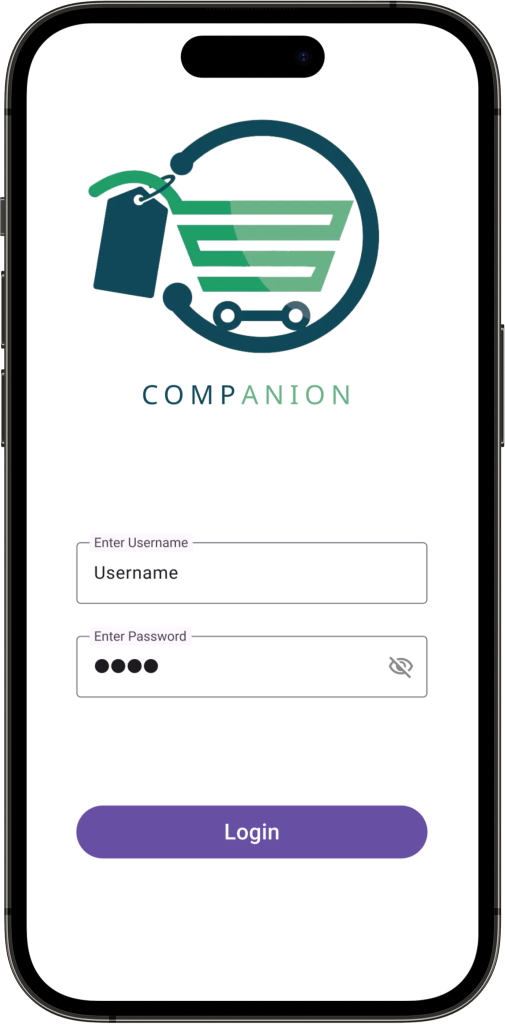
\includegraphics[width=\ImageSize\linewidth]{Assets/Login mockup.png}
    \caption{Pagina di Login}
    \label{login_figma}
\end{figure}
\noindent

\newpage
\subsubsection{Home}
La schermata Home è la pagina principale che compare quando si è eseguito il login. Come richiesto dal tutor aziendale è caratterizzata da una barra di ricerca, che contiene al suo interno anche un pulsante per aprire il Drawer, una lista con i prodotti ricercati e un pulsante per andare alla pagina del carrello. Le Card \cite{card} della lista sono composte da un immagine facoltativa (a seconda se il Server la rende disponibile o meno), del testo che descrive il prodotto con relativo codice e un pulsante adibito all'aggiunta nel carrello. L'immagine di sfondo compare in caso di lista vuota ed è stata inserita a scopo di riempimento.
\begin{figure}[h]
\centering
	\begin{minipage}[t]{\ImageSize\linewidth}
		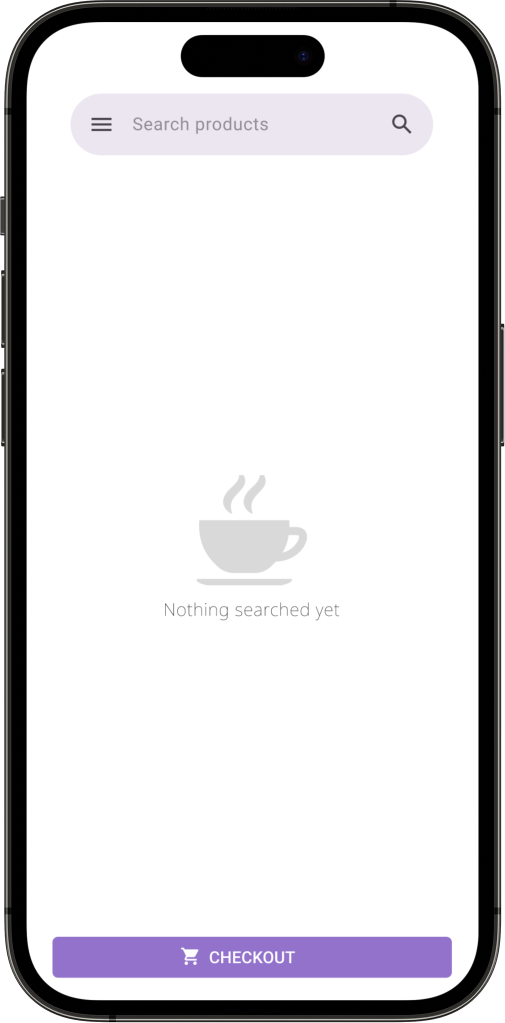
\includegraphics[width=\linewidth]{"Assets/Empty mockup.png"}
		\caption{Pagina Home con ricerca}
		\label{fig:figma_home}
	\end{minipage}
	\hspace{1em}
	\begin{minipage}[t]{\ImageSize\linewidth}
		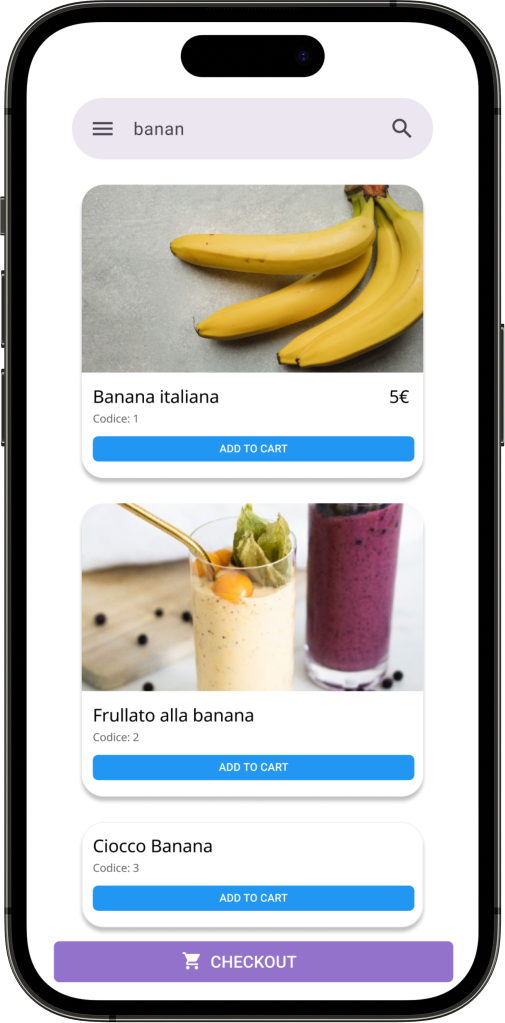
\includegraphics[width=\linewidth]{"Assets/List mockup.png"}
	\end{minipage}

\end{figure}

\newpage
\subsubsection{Carrello}
La pagina del carrello presenta anch'essa una disposizione in forma di lista e, in conformità alle direttive dettate dal mio supervisore aziendale, ogni Card di essa offre la possibilità di modificare la quantità di ciascun articolo tramite specifici pulsanti, consentendo inoltre di eliminare ogni singolo elemento dal carrello mediante uno swipe verso sinistra. Si provvede altresì a indicare il prezzo unitario di ciascun prodotto insieme all'importo totale corrispondente alla quantità selezionata. Infine, nella parte inferiore della pagina, è presente un pulsante dedicato all'invio dell'ordine, accompagnato dal riepilogo del prezzo totale.
\begin{figure}[H]
    \centering
    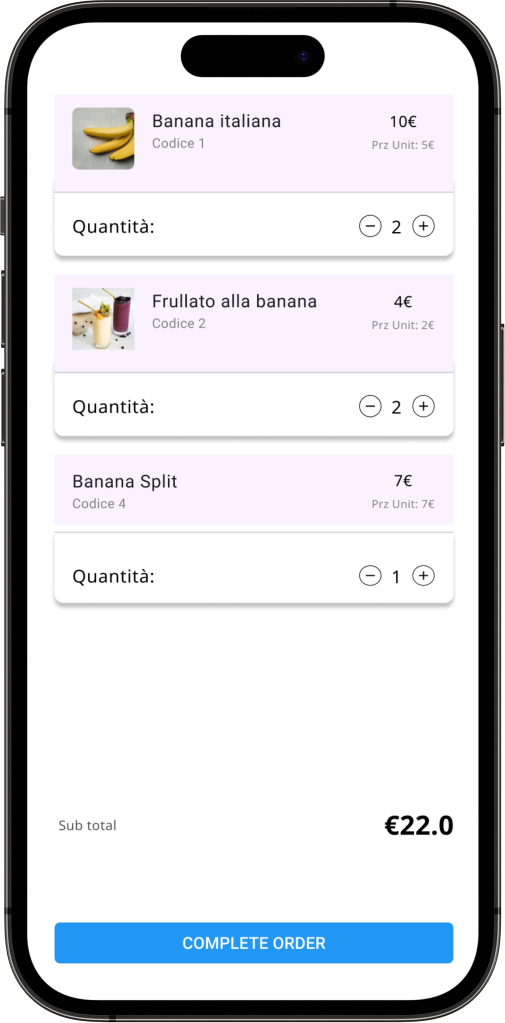
\includegraphics[width=\ImageSize\linewidth]{Assets/Cart mockup.png}
    \caption{Pagina del Carrello}
    \label{fig:figma_cart}
\end{figure}

\newpage
\subsubsection{Profilo}
La pagina del profilo è stata creata per mostrare le informazioni dell'utente. Avendo a disposizione di pochi dati da mostrare, ho deciso di optare per una soluzione a "lista" che mostra giusto le informazioni essenziali spezzando il più possibile a fini di riempimento (per esempio la divisione tra nome e cognome in 2 campi di testo diversi è voluta)
\begin{figure}[H]
\centering
	\begin{minipage}[t]{\ImageSize\linewidth}
		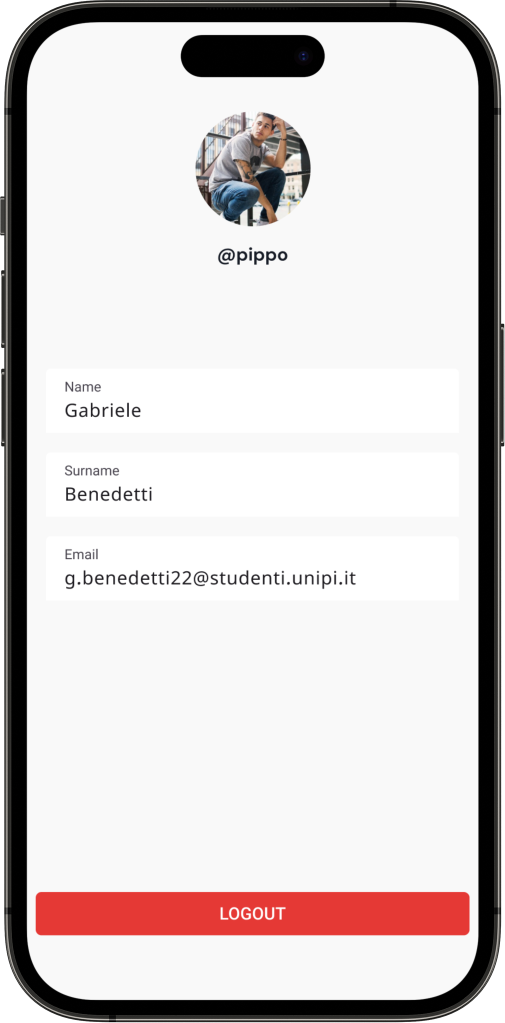
\includegraphics[width=\linewidth]{"Assets/mockup image.png"}
	\end{minipage}
	\hspace{1em}
	\begin{minipage}[t]{\ImageSize\linewidth}
		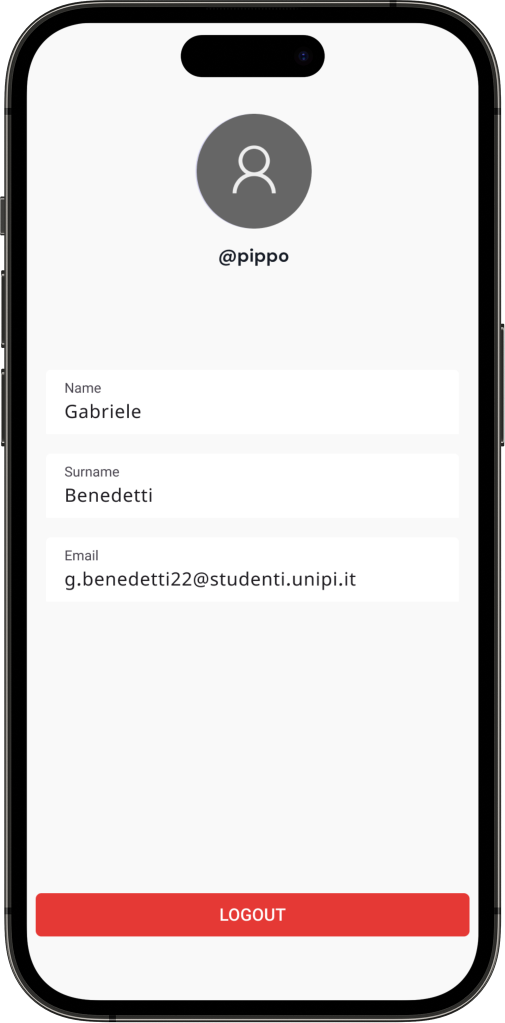
\includegraphics[width=\linewidth]{"Assets/mockup no image.png"}
	\end{minipage}
	\captionof{figure}{Pagina del Profilo utente}
	\label{fig:figma_profile}
\end{figure}


\subsection{Da Figma a Flutter - Sviluppo della UI}
Tutte le schermate dell'applicazione sono state inserite dentro uno Scaffold. L'AppBar inclusa è comune a tutte le schermate, contenente un titolo e una barra di caricamento richiamabile mediante Provider (vedi \Cref{lab_widget_communication}).\\
Nelle sezioni successive verrà menzionato notevolmente anche il Widget Expanded, quindi il lettore è richiamato a rileggere la \Cref{subsub:expanded} in caso non si abbia chiaro a cosa serva questo Widget.
Infine vorrei sottolineare che i frammenti di codice inseriti sono da considerarsi più come strumento per capire la logica adottata dietro la costruzione dell'interfaccia, infatti molte cose verranno tralasciate poiché considerate irrilevanti.

\subsubsection{Login}
In accordo con quanto stabilito nella \Cref{login_figma}, la pagina di Login deve contenere un immagine, 2 campi di testo e un pulsante per inoltrare la richiesta di accesso.
Essendo a tutti gli effetti un form è stato quindi usata la classe Form che Flutter mette a disposizione: questo Widget permette la validazione dei campi tramite callbacks\footnote{una funzione che viene passata come parametro e poi eseguita in seguito} e l'uso di TextFormField che incorporano dei messaggi di errore in caso l'utente inserisca dei dati sbagliati. Di seguito lo pseudo-codice:
\begin{lstlisting}[language=Java, firstnumber=1][H]
TextEditingController usernameController, passwordController;
GlobalKey<FormState> formKey;

Column(
	children: [
		Expanded (
			child : Image.asset("logo.png"),
		),
		Expanded(
			child : Form(
				key : formKey, // per tenere un riferimento al form
				child : Column(
					children : [
						TextFormField(
							controller: usernameController,
						),
						TextFormField(
							controller: passwordController
						)
					]
				)
			)
		),
		Expanded(
			child : ElevatedButton(
				onPressed : () {
					String username = usernameController.text;
					String password = passwordController.text;
					login(username, password);
				},
				child : Text("Login"),
			)
		),
	],
)
\end{lstlisting}
A questo punto i dati del Form devono avere una qualche "regola di verifica" quando l'utente preme il pulsante di autenticazione. Per farlo, possiamo quindi passare una "callback" all'oggetto "TextFormField" e questa callback avrà, come parametro la stringa presente nel campo di testo e deve restituire "null" se tutto è corretto, altrimenti un messaggio di errore che verrà mostrato all'utente nel corrispettivo TextFormField. Il codice deve essere quindi modificato secondo quanto segue:
\begin{lstlisting}[language=Java, firstnumber=9][H]
child : Form(
	key : formKey,
	child : Column(
		children : [
			TextFormField(
				controller: usernameController,
				validator: (value) => isUsernameValid(value),
			),
			TextFormField(
				controller: passwordController,
				validator: (value) => isPasswordValid(value),
			)
		]
	)
)

// ritorna null se username e' ok, il messaggio di errore altrimenti
String? isUsernameValid(String? username) {
	if (username == null) 
	 return "Username cannot be null";
	 
	if (username.trim().isEmpty)
	 return "Username cannot be empty";
	 
	if (username.isEmpty)
	 return "Username cannot be only whitespaces";
	 
	if (username.contains(" "))
	 return "Username can't contain spaces";
	
	return null;
}

// ritorna null se password e' ok, il messaggio di errore altrimenti
String? isPasswordValid(String? password) {
	if (password == null)
	 return "Password cannot be null";
	 
	if (password.isEmpty)
	 return "Password cannot be empty";
	 
	if (password.trim().isEmpty)
	 return "Password cannot be only whitespaces";
	
	return null;
}
\end{lstlisting}

\noindent
Infine, per effettuare effettivamente la convalida del form, sarà necessario implementare la funzione di login. Basterà tuttavia chiamare il metodo "validate()", tramite la formKey definita globalmente, che attiverà le callback descritte prima e poi restituirà "true" se i dati sono validi, "false" altrimenti.\\ In codice:
\begin{lstlisting}[language=Java, firstnumber=1][H]
	void login(String username, String password) async {
		if (formKey.currentState!.validate()) {
			// form valido
		}
	}
\end{lstlisting}

\noindent
\subsubsection{Home} \label{subsub:home}
In accordo con quanto mostrato in \Cref{fig:figma_home} la pagina Home consiste in una SearchBar, che l'utente può usare per ricercare i prodotti e aprire il Drawer, una lista e un pulsante per andare alla pagina del carrello (di cui non approfondirò essendo un semplice pulsante con applicato dello stile). Questi 3 componenti sono stati sviluppati separatamente e inclusi all'interno di un Widget Column\footnote{Widget Flutter per disporre gli elementi in modo verticale} affinché stiano uno sotto l'altro. In codice:
\begin{lstlisting}[language=Java, firstnumber=1][H]
Column (
	children : [
		CompanionSearchBar(),
		ProductsList(),
		GotoCartButton()
	]
)
\end{lstlisting}

\newpage
\paragraph{CompanionSearchBar}

\noindent
Come è facile intuire dal nome, la SearchBar è stata ricreata da zero utilizzando un TextField standard, invece di impiegare il Widget di base fornito da Flutter: questo perchè la SearchBar nativa non fornisce la possibilità di passare una callback richiamabile quando l'utente preme il pulsante di invio sulla tastiera (fisica o virtuale), bensì è presente la sola possibilità di inserire una callback quando l'utente immette un qualsiasi carattere alfa-numerico o carattere speciale. Questa mancanza non mi ha permesso di poter gestire adeguatamente la ricerca dei prodotti, soprattutto a livello di efficienza in quanto eseguire una richiesta per carattere immesso richiede un uso sconsiderato delle risorse.\\
La CompanionSearchBar è dotata di un Hamburger menù richiamabile mediante l'apposita icona di prefisso e un ulteriore icona di suffisso che cambia in base a se l'utente sta scrivendo oppure no: se è presente del testo allora l'icona sarà funzionale e di pulitura (cioè l'utente può cliccarci per pulire il TextField) altrimenti viene mostrata l'icona base di ricerca che è fittizia. Questa implementazione non è nel mockup ed è stata decisa in fase di sviluppo per richiamare l'esperienza offerta dalle app mobile simili più famose, garantendo un senso di familiarità agli utenti. In codice:
\begin{lstlisting}[language=Java, firstnumber=1][H]
TextEditingController controller = TextEditingController();
bool isTyping = false;

TextField(
	controller: controller,
	textInputAction: TextInputAction.search,
	onSubmitted: (value) {
		setState(() {
			isTyping = false;
			// se sono presenti solo spazi bianchi
			if (value.trim().isEmpty) {
				return;
			}
			search(value); // esegui ricerca
		});
	},
	onTap: () { // quando l'utente comincia a digitare..
		setState(() {
			isTyping = true;
		});
	},
	decoration: InputDecoration(
		prefixIcon: IconButton(
			icon: const Icon(Icons.menu_outlined),
			onPressed: () {
				// aprire Drawer menu
			}
		),
		// se l'utente sta digitando allora mostra l'icona di
		// pulitura, altrimenti quella di ricerca
		suffixIcon: isTyping ? IconButton(
			icon: const Icon(Icons.clear),
			onPressed: () {
				controller.clear();
			}) : const Icon(Icons.search)
		)
	)
)

\end{lstlisting}

\noindent
\paragraph{Drawer}
Nelle specifiche dell'applicazione è richiesto anche che sia incluso un Drawer richiamabile, come detto sopra. Questo Widget si può includere dentro lo Scaffold e rappresenta una lista a comparsa contenente opzioni che l'utente può scegliere, in particolare quelle richieste sono:
\begin{itemize}
	\item Visualizzazione del Profilo
	\item Cronologia delle testate
	\item Logout
\end{itemize}
Il Drawer si può quindi creare nel seguente modo:
\begin{lstlisting}[language=Java, firstnumber=1][H]
Scaffold(
	drawer: Drawer(
		child: ListView(
			children: [...]
		)
	)
)
\end{lstlisting}

\noindent
Gli elementi del Drawer sono principalmente dei ListTile\footnote{Un Widget di Flutter che corrisponde, solitamente, a del testo con un icona posizionata alla sua sinistra}, accompagnati da un DrawerHeader\footnote{Un Widget di Flutter che corrisponde al primo elemento del Drawer. Solitamento è meso come abbellimento in quanto corrisponde quasi sempre ad un immagine} come primo elemento a scopo puramente estetico. In particolare il DrawerHeader è così composto:
\begin{lstlisting}[language=Java, firstnumber=50][H]
children: [
	DrawerHeader(
		child: Image.asset("logo.png")
	)
]
\end{lstlisting}

\newpage
\noindent
Mentre i ListTile hanno tendenzialmente questa struttura:
\label{cod:listile}
\begin{lstlisting}[language=Java, firstnumber=58][H]
ListTile(
	leading: const Icon(...),
	title: const Text("title"),
	onTap: () {
		// azione da eseguire...
	}
)
\end{lstlisting}

\noindent
Quindi, in conclusione, il Drawer è così composto:
\begin{lstlisting}[language=Java, firstnumber=1][H]
Scaffold(
	drawer: Drawer(
		child: ListView(
			children: [
				DrawerHeader(
					child: Image.asset("logo.png")
				),
				ListTile(
					leading: const Icon(...),
					title: const Text("title"),
					onTap: () {
						// azione da eseguire...
					}
				),
				... // altri ListTile
			]
		)
	)
)
\end{lstlisting}

\noindent
Ed è richiamabile mediante la funzione:
\begin{lstlisting}[language=Java, firstnumber=1][H]
	Scaffold.of(context).openDrawer();
\end{lstlisting}

\noindent
\paragraph{Lista dei prodotti ricercati} \label{par:listview}
Per quanto riguarda la lista dei prodotti, è stata adottata la componente nativa di Flutter denominata ListView, costruita mediante il metodo "ListView.builder()".
Come richiesto, i componenti della lista sono delle Material Card che a loro volta sono composte da un immagine facoltativa (a seconda se il Server la restituisce oppure no), una descrizione del prodotto, il relativo codice, il prezzo unitario di vendita e un pulsante per aggiungere al carrello il prodotto desiderato. Flutter mette a disposizione un Widget nativo chiamato appunto "Card" che permette la creazione di questi elementi dalla forma particolare. In codice:
\begin{lstlisting}[language=Java, firstnumber=1][H]
child: Card(
	shape: RoundedRectangleBorder(
		borderRadius: BorderRadius.circular(radius),
	)
	child: ...
)
\end{lstlisting}

\noindent
Così facendo le Card hanno il bordo arrotondato proprio come nel mockup. Per gli altri elementi è stato usato un Widget di tipo Column e uno di tipo Row\footnote{Widget di Flutter per disporre gli elementi in modo orizzontale da sinistra verso destra} per avere la descrizione del titolo e il prezzo uno di fianco all'altro. Per aiutare il lettore nella comprensione di quanto scritto, inserisco un immagine esplicativa:
\begin{figure}[H]
\centering
	\begin{minipage}[t]{0.45\linewidth}
		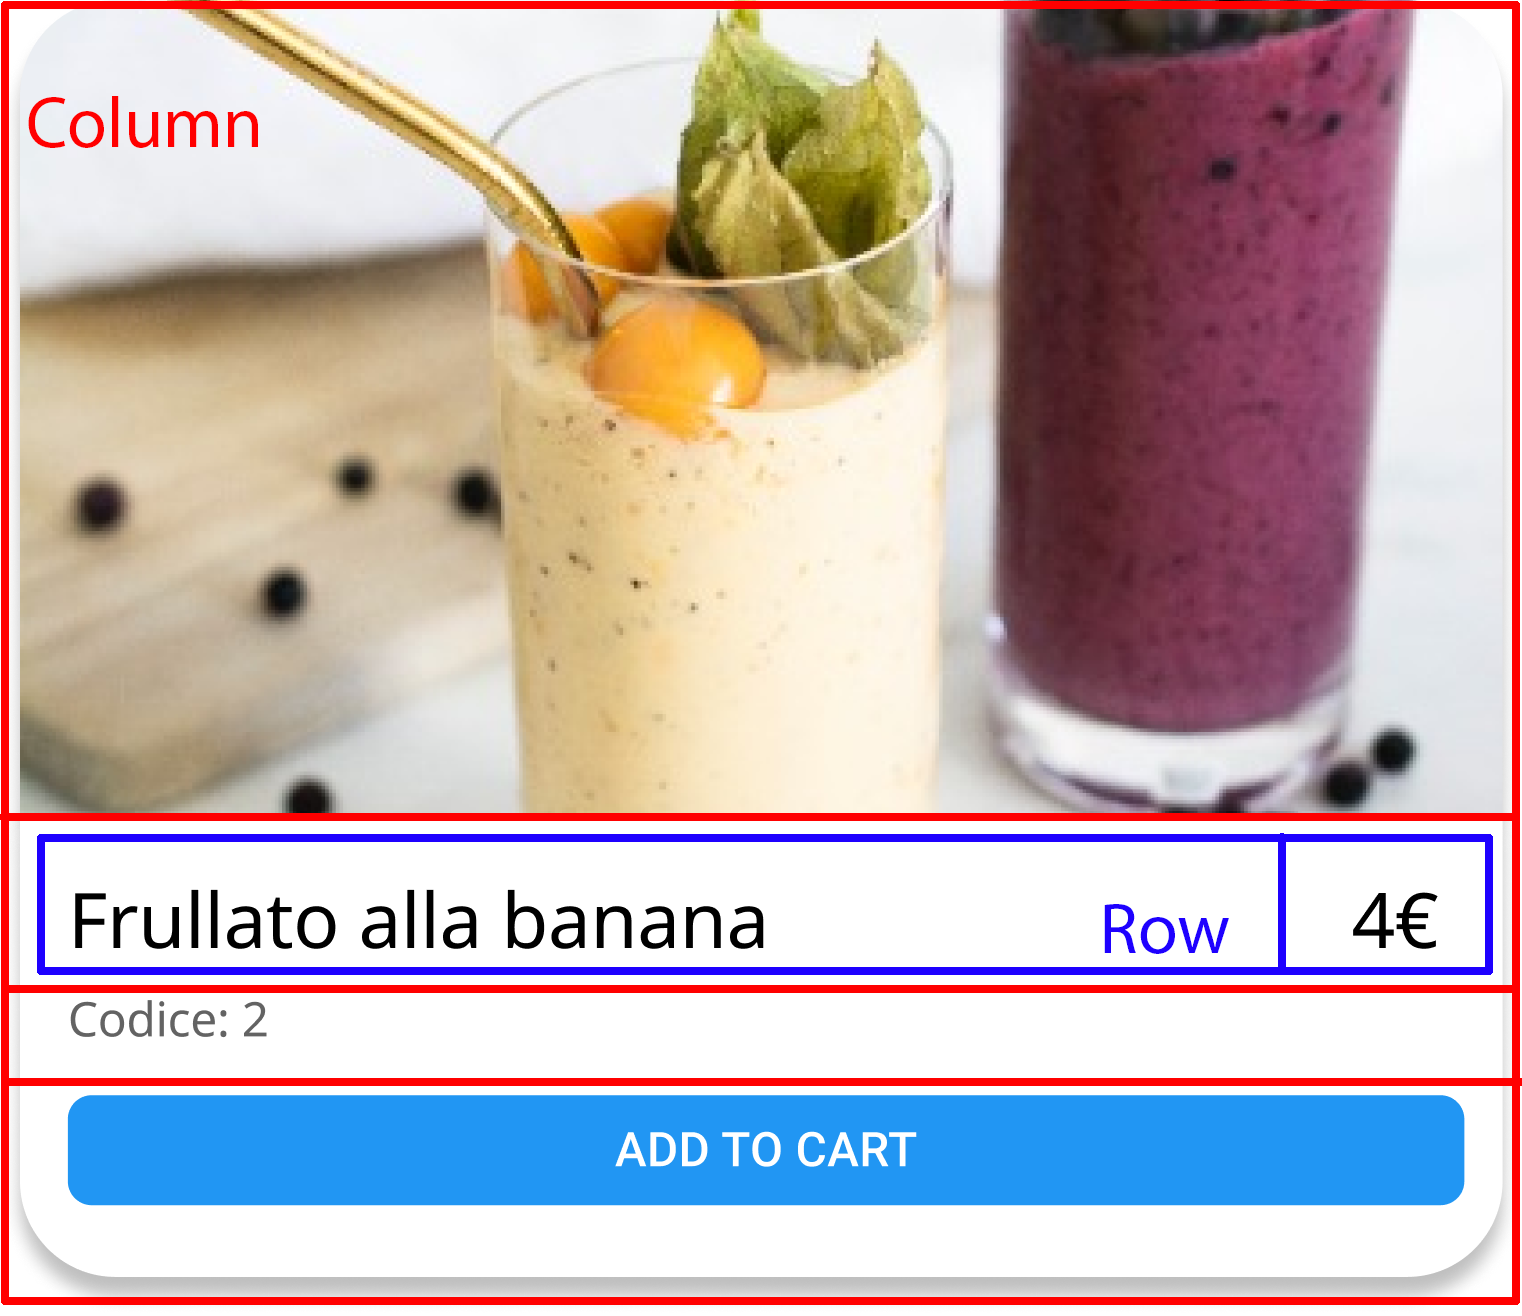
\includegraphics[width=\linewidth]{"Assets/card explained.png"}
	\end{minipage}
\end{figure}
Quindi dentro Column devono andare: la copertina se presente, Il Widget Row, che contiene a sua volta la descrizione e il prezzo unitario di vendita, l'id del prodotto e infine il pulsante. In pseudo-codice:
\begin{lstlisting}[language=Java][H]
Column(
	children: [
		if(url != null)
			Image.network(image_url),
		Row(
			children: [
				Text(desc),
				Text(price)
			]
		),
		Text(productId),
		RoundedLoadingButton(
			child: Text("ADD TO CART"),
			onPressed: () {
				// aggiungi al carrello
			}
		)
	]
)
\end{lstlisting}

\noindent
\subsubsection{Carrello}
Come è facile notare dalla \Cref{fig:figma_cart}, questa schermata presenta molte somiglianze con la pagina Home, in quanto ospita un elenco dinamico di Card. In aggiunta, vengono mostrati dettagli dell'importo totale e un pulsante per inoltrare l'ordine nella parte inferiore della schermata. Tuttavia, in questa situazione, le "Card" sono più complesse e richiedono un numero maggiore di elementi grafici anche se ci sono molte anolgie con le Card della schermata Home. La pagina è stata quindi divisa in questo modo
\begin{lstlisting}[language=Java, firstnumber=1][H]
Column (
	children : [
		ProductsList(),
		SubTotalAmount()
	]
)
\end{lstlisting}

\noindent
\paragraph{ProductsList}
Questa lista è molto simile a quella già descritta nella \Cref{par:listview}, ma il cambiamento principale sta proprio nelle Card: oltre ai soliti dati, quali descrizione del prodotto, codice, immagine facoltativa e prezzo unitario, è stata aggiunta la possibilità di modificare la quantità mediante 2 appositi pulsanti circolari insieme ad una label che mostra il prezzo totale dell'ordine (che corrisponde al prezzo unitario per la quantità). Inoltre i dati già descritti sono stati inseriti dentro un ListTile (vedi \Cref{cod:listile}). Per agevolare la comprensione al lettore, allego un'immagine esplicativa che illustra la progettazione dell'interfaccia utente in modo più semplice e chiara:
\begin{flushleft}
	\begin{minipage}[t]{1\linewidth}
		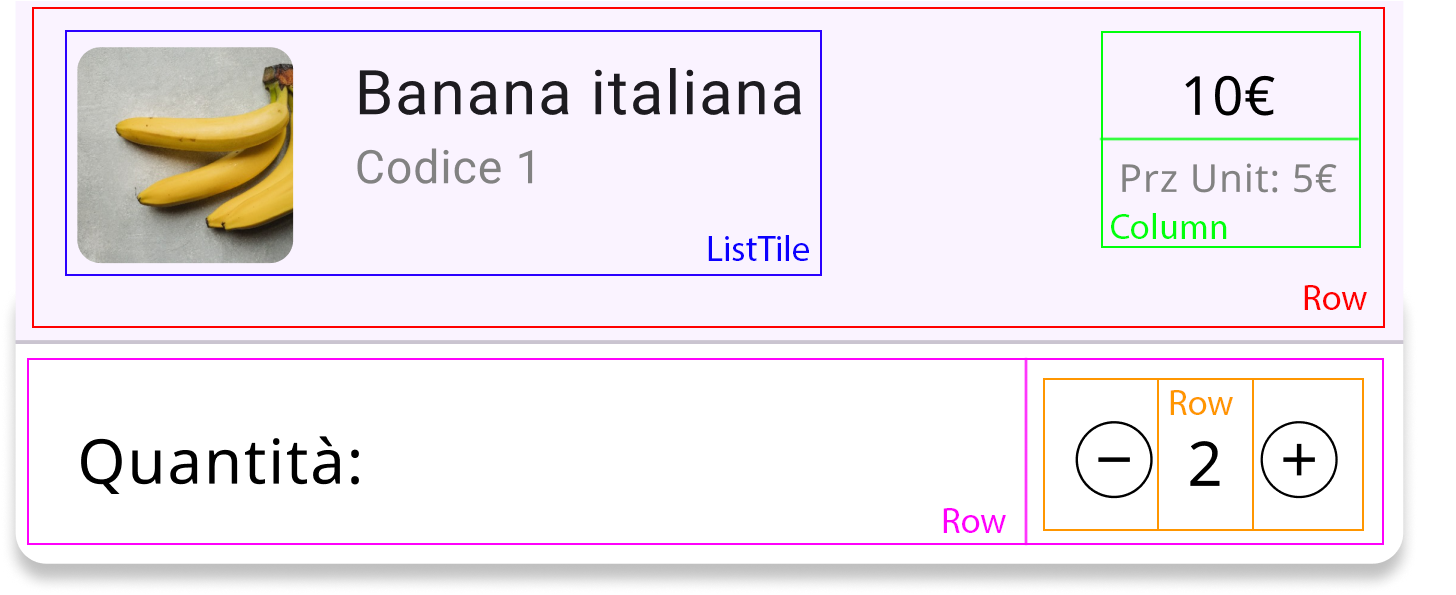
\includegraphics[width=\linewidth]{"Assets/complex list item.png"}
		\label{fig:complexCard}
	\end{minipage}
\end{flushleft}

\noindent
In codice:
\begin{lstlisting}[language=Java, firstnumber=1][H]
Column(
	children: [
		Row(
			children: [
				Expanded(
					ListTile(...),
				),
				Column(
					children: [
						Text(price),
						Text(priceUnit),
					]
				)
			
			]
		),
		Row(
			children: [
				Expanded(
					Text("Quantity"),
				),
				Row(
					children: [
						IconButton(...), // aggiungi quantita'
						Text(quantity),
						IconButton(...), // rimuovi quantita'
					]
				)
			]
		)
	]
)
\end{lstlisting}

\noindent
Piccola nota di rilievo va al ListTile (quadrato blu della figura sopra) che è stato sviluppato come segue:
\begin{lstlisting}[language=Java, firstnumber=122][H]
ListTile(
	leading: imgUrl != null ? Image.network(umgUrl) : null,
	title: const Text(desc),
	subtitle: const text(productId)
)
\end{lstlisting}

\noindent
Mentre la label "Quantità" della \Cref{fig:complexCard} è stata inserita dentro un Widget Expanded in modo che la seconda riga, quella che contiene i pulsanti per modificare la quantità, si spostasse tutta a destra.
Queste Card hanno infine la peculiarità di essere dismissible: l'utente può trascinare verso sinistra o destra una di esse per rimuovere l'ordine dal carrello. Per far ciò basta inserire la Card dentro un Widget di tipo Dismissible, in questo modo:
\begin{lstlisting}[language=Java, firstnumber=1][H]
Dismissable(
	child: Card(...)
)
\end{lstlisting}

\noindent

\paragraph{SubTotalAmount}
La parte dedicata al display del prezzo totale occupa una porzione fissa all'interno della schermata: di fatto, allo scorrere della lista, questa non si muove con essa. Lo sviluppo è molto semplice, di fatto è una Row (che contiene le due label "Sub-Total" e il prezzo, vedi \Cref{fig:figma_cart}) dentro un Widget Column. In codice:
\begin{lstlisting}[language=Java, firstnumber=1][H]
Column(
	children: [
		Row(
			children: [
				Expanded(
					child: Text("Sub Total"),
				),
				Expanded(
					child: Text(totalPrice)
				)
			]
		)
	],
	ElevatedButton(
		child: Text("Submit Order")
	)
)
\end{lstlisting}

\noindent
\subsubsection{Profilo}
Come illustrato in \Cref{fig:figma_profile}, la schermata del profilo presenta un'immagine con il relativo username posizionato appena sotto di essa. Le informazioni dell'utente sono organizzate in una breve lista, e vi è un pulsante "logout" di colore rosso. Ho scelto di adottare questa disposizione poiché le informazioni disponibili nel Database sono limitate, e ho cercato quindi di ottimizzare l'utilizzo dello spazio a mia disposizione. In realtà, con ulteriori informazioni, potrebbe essere opportuno considerare l'opzione di unire i campi "nome" e "cognome" in un'unica etichetta.\\
Nota: è importante precisare che l'indirizzo email e la foto del profilo vengono attualmente inseriti a scopo illustrativo e non sono effettivamente ricevuti dal Server. In codice:
\begin{lstlisting}[language=Java, firstnumber=1][H]
Expanded(
	child: Column(
		children: [
			Expanded(
				flex: 1,
				ClipOval(
					child: FadeInImage(
						image: const NetworkImage(url),
						imageErrorBuilder: (context, error, stackTrace) {
							return const CircleAvatar(
								backgroundImage: AssetImage("profile.png")
							);
						}
					)
				),
				Text(username),
			),
			Expanded(
				flex: 2,
				child: Column(
					children: [
						Text(name),
						Text(surname)
					]
				)
			),
			Expanded(
				child: ElevatedButton(child: Text("LOGOUT"))
			)
		]
	)

)	
\end{lstlisting}

\noindent
Un dettaglio da sottolineare riguarda l'utilizzo dei valori "flex: 1" e "flex: 2". Questi parametri definiscono la quantità di spazio che i Widget sono autorizzati a occupare all'interno del layout. Di norma, tutti i Widget hanno un valore predefinito di "flex: 1", il che significa che si distribuiranno equamente nello spazio disponibile. La lista, tuttavia, che visualizza le informazioni dell'utente, richiede più spazio rispetto all'immagine e al testo sottostante posizionati nella parte superiore della pagina, per questo le è assegnato un valore "flex: 2". Per approfondire meglio invece l'utilizzo di "FadeInImage", rimando il lettore al \Cref{subsub:fadeinimage}.

\subsection{Comunicazione tra Widget} \label{lab_widget_communication}
Per la comunicazione tra i vari Widget viene utilizzata la classe "SharedProvider" (vedi \Cref{subsub:provider}). Essa assume un ruolo di rilievo nell'orchestrare la comunicazione efficace tra i Widget Flutter. In particolare, la sua funzione centrale è quella di facilitare la condivisione di dati e lo scambio di informazioni tra diverse parti dell'applicazione, contribuendo a mantenere uno stato coerente e sincronizzato tra i vari componenti.\\
In particolare questa classe memorizza:
\begin{itemize}
	\item Token di accesso e aggiornamento,
	\item Carrello utente,
	\item Articoli cercati dall'utente che sono restituiti dal Server,
	\item Testata corrente,
	\item Importo complessivo dei prodotti presenti nel carrello.
\end{itemize}

\noindent
\paragraph{Creazione di SharedProvider}
Questa classe estende ChangeNotifier della libreria Provider e la sua creazione avviene all'avvio dell'applicazione subito dopo il main:
\begin{lstlisting}[language=Java, firstnumber=1][H]
	void main() {
		runApp(const CompanionApp());
	}
	
	class CompanionApp extends StatefulWidget {
		const CompanionApp({super.key});
		
		@override
		State<CompanionApp> createState() => CompanionAppState();
	}
	
	class CompanionAppState extends State<CompanionApp> {

		@override
		Widget build(BuildContext context) {
			return MultiProvider(
			providers: [
				ChangeNotifierProvider(
					create: (.) => SharedProvider()
				),
			],
			...
		}
\end{lstlisting}

\noindent
A questo punto il Provider è disponibile in qualsiasi punto dell'applicazione, richiedibile mediante:
\begin{lstlisting}[language=Java, style=longBlock, firstnumber=1][H]
	SharedProvider p = Provider.of<SharedProvider>(context, listen: false);
	
	// in caso non sia disponibile il contesto context:
	WidgetsBinding.instance.addPostFrameCallback((timeStamp) {
		SharedProvider provider = Provider.of<SharedProvider>(context, listen: false);
	});
\end{lstlisting}

\noindent
Per semplicità e compattezza, è stato implementato un metodo statico (detto anche "stub") all'interno della classe SharedProvider. Questo metodo è stato progettato appositamente per agevolare l'accesso al Provider in maniera diretta e immediata, richiedendo solamente il parametro di tipo BuildContext\footnote{Classe astratta di Flutter che rappresenta il cuore di un Widget. Un BuildContext in Flutter è un oggetto che fornisce informazioni sulla posizione di un Widget all'interno del "Widget Tree". È essenziale per accedere a risorse e dati specifici del Widget, infatti ogni Widget è associato ad un BuildContext.}:
\begin{lstlisting}[language=Java][H]
factory SharedProvider.getInstance(BuildContext context) {
	return Provider.of<SharedProvider>(context, listen: false);
}
\end{lstlisting}

\noindent
\paragraph{Caricamento dei dati}
All'avvio dell'applicazione vengono lette e caricate le informazioni utente dal disco fisico dentro la classe SharedProvider poichè questa operazione assicura che, durante l'intero ciclo di vita dell'applicazione, le informazioni necessarie per il suo corretto funzionamento siano prontamente accessibili. In pseudo-codice:
\begin{lstlisting}[language=Java, firstnumber=1][H]
Map<String, Object> initData = loadFromDisk();

String accessToken = initData['access_token'];
String refreshToken = initData['refresh_token'];
int currentTestataId = initData['currentTestataId'];
List<Order> cart = initData['cart'];

SharedProvider provider = SharedProvider.getInstance(context);
provider.accessToken = accessToken;
provider.refreshToken = refreshToken;
provider.currentTestataId = currentTestataId;
provider.cartProducts = cart;
\end{lstlisting}

\noindent
Un esempio concreto è la situazione in cui vi sia la necessità di recuperare il token di accesso. In tal caso, basta seguire la sequenza di istruzioni di seguito riportata:
\begin{lstlisting}[language=Java, firstnumber=1][H]
SharedProvider provider = SharedProvider.getInstance(context);

const accessToken = provider.accessToken;
\end{lstlisting}

\noindent
\paragraph{Aggiornamento UI}
Per fare in modo che gli elementi dell'interfaccia utente si aggiornino quando si verificano dei cambiamenti, è essenziale inserirli nell'oggetto di tipo "Selector" (vedi \Cref{subsub:provider}). Un esempio può essere l'aggiornamento del prezzo totale della testata ogni qual volta l'utente inserisce un prodotto nuovo al carrello o modifica la quantità di un ordine:
\begin{lstlisting}[language=Java, firstnumber=1][H]
	child: Selector<SharedProvider, double>(
		selector: (context, provider) => provider.cartTotalPrice,
		builder: (context, cartTotalPrice, child) {
			return Text(cartTotalPrice);
		}
	)
\end{lstlisting}

\noindent
In questo caso, il parametro "selector" prende in input il prezzo totale del carrello cosicché, quando questo cambia, la funzione passata al parametro "builder" venga usata per aggiornare l'interfaccia utente con il nuovo dato.
Per notificare il cambiamento, basta invocare il metodo:
\begin{lstlisting}[language=Java, firstnumber=1][H]
	notifyListeners();
\end{lstlisting}

\noindent
ereditato dalla classe ChangeNotifier. Sempre in riferimento all'esempio mostrato sopra, quindi, per aggiornare il prezzo totale della testata basta inserire dentro la classe SharedProvider:
\begin{lstlisting}[language=Java, firstnumber=1][H]
	void setTotalPrice(double price) {
		cartTotalPrice = price;
		notifyListeners();
	}
\end{lstlisting}

\noindent
A questo punto, una volta invocato il metodo sopra, il Selector noterà la differenza con il valore precedente e invocherà la funzione passata al parametro "builder" per aggiornare l'interfaccia.\\
Questo approccio assicura un notevole livello di efficienza e contribuisce a una drastica riduzione del consumo energetico, un aspetto di cruciale importanza nel contesto dello sviluppo di applicazioni mobili. Inoltre viene ridotto significativamente il carico computazionale richiesto per aggiornare la UI, poiché vengono evitate le ricostruzioni inutili e, di conseguenza, si riscontra una diminuzione sostanziale nell'utilizzo di risorse, tra cui CPU e memoria (ciò è particolarmente rilevante nei dispositivi mobili, dove le risorse sono spesso limitate). Infine, l'adozione di tale approccio consente di garantire una risposta più rapida agli aggiornamenti dei dati, poiché solo le porzioni rilevanti dell'interfaccia vengono adeguatamente aggiornate.\\ Questo si traduce in un'esperienza utente più fluida e reattiva, contribuendo a migliorare la percezione complessiva dell'applicazione da parte degli utenti.

\subsection{Asincronia delle richieste}
L'applicazione fa un ampio utilizzo delle chiamate asincrone, poiché spesso è necessario comunicare con il Server e, attendere sempre la risposta, causerebbe un blocco totale dell'applicazione, il che è altamente irrealistico. Tuttavia, sorge il problema che in molte occasioni è necessario visualizzare un'interfaccia ancor prima di aver ottenuto i dati necessari per popolarla.
Per superare questa difficoltà, Flutter mette a disposizione il Widget FutureBuilder, che è stato impiegato per presentare all'utente un'interfaccia predefinita mentre si attende il completamento del caricamento dei dati dal Server. Un esempio concreto si manifesta nella pagina del carrello: fintanto che l'elenco dei contenuti corretto non è disponibile, viene mostrato l'ultimo elenco ricevuto salvato localmente. Il seguente codice ne rappresenta un esempio:
\begin{lstlisting}[language=Java, style=longBlock, firstnumber=1][H]
body: FutureBuilder<List<Order>>(
		future: getCart(),
		initialData: SharedProvider.getInstance(context).cartProducts,
		builder: (context, snapshot) {
			if (!snapshot.hasData) {
				return const LoadingPage();
			}
			
			// lista pronta
			List<Order> list = snapshot.data;
		}
	)
	
Future<List<Order>> getCart() async {
	// richiesta HTTP per prendere il carrello in modo asincrono
}
\end{lstlisting}

\noindent
Nell'esempio sopra, si evidenzia la potenza del FutureBuilder: mentre il carrello viene recuperato dal Server attraverso la funzione "getCart()", il Widget utilizza dati iniziali per mostrare istantaneamente "qualcosa" all'utente. Questo "qualcosa" corrisponde alla lista più recente di ordini ricevuta dal Server e memorizzata localmente (tutto ciò avviene senza interferire con il processo di scaricamento in background). In questo contesto, il valore "snapshot.data" rappresenta l'initialData, ossia la lista locale e, una volta che il Client riceve effettivamente il carrello, il FutureBuilder invoca il metodo definito nel parametro "builder" con lo snapshot che conterrà i dati scaricati attraverso il metodo "getCart()", anziché i dati locali precedentemente visualizzati. L'if è stato messo a scopo difensivo, in quanto è possibile che non esista nessuna lista localmente e che il tempo di scaricamento sia prolungato.\\
Per concludere, un ulteriore e importante strato di asincronia è stato adottato nell'esecuzione delle richieste HTTP, con incluse le relative gestioni dei timeout. Queste operazioni avvengono in background, una scelta guidata dalla necessità di ottimizzare le performance complessive dell'applicazione. L'interfaccia tra l'app e il protocollo HTTP è stata gestita attraverso la classe astratta "NetworkUtility": questo oggetto non solo esegue i controlli per la validità dei token (in più, nel caso in cui il token di accesso sia scaduto, la classe ne richiederà immediatamente, al Server, uno nuovo) prima di inoltrare la richiesta, ma si occupa anche di presentare eventuali messaggi di errore all'utente mediante l'uso di material dialog.

\subsection{Persistenza su disco}
Per quanto riguarda la memorizzazione delle informazioni dell'utente e dell'ultimo carrello ricevuto dal Server, è stato adottato il framework SQLite. Tali dati vengono archiviati su disco all'interno di apposite tabelle, create appositamente per questa finalità. La struttura del Database è generata secondo la seguente procedura:
\begin{lstlisting}[language=SQL, style=longBlock, firstnumber=1][H]
    openDatabase(
        join(await getDatabasesPath(), 'companion.db'),
        version: 1, onCreate: (db, version) async {
      await db.execute(
        'CREATE TABLE User(id INTEGER PRIMARY KEY, name TEXT, surname TEXT, creationDate TEXT, username TEXT)');
      return db.execute(
        'CREATE TABLE Products(id INTEGER PRIMARY KEY, desc TEXT, price REAL, quantity INTEGER, imageUrl TEXT)',
      );
    });
\end{lstlisting}

\noindent
Ora è intuitivo concepire che le informazioni dell'utente siano conservate nella prima tabella denominata "User", mentre i prodotti nel carrello trovano collocazione nella seconda tabella chiamata "Products". Dato che è necessario archiviare oggetti all'interno del Database, ho seguito il consiglio proveniente dalla documentazione di Flutter, pertanto, ho implementato due metodi che permettono la conversione dell'oggetto in una struttura di tipo mappa (Map) e la successiva ricostruzione dell'oggetto a partire da questa. Il procedimento si articola nel seguente modo:
\newpage
\begin{lstlisting}[language=Java, firstnumber=1][H]
class User {
  final String name;
  final String surname;
  final String creationDate;
  final String username;

  User(this.name, this.surname, this.creationDate, this.username);

  factory User.fromMap(Map<String, dynamic> json) {
    return User(
      json['name'],
      json['surname'],
      json['creationDate'],
      json['username'],
    );
  }

  Map<String, Object?> toMap() {
    return {
      "name" : name,
      "surname" : surname,
      "creationDate" : creationDate,
      "username" : username,
    };
  }
}
\end{lstlisting}

\noindent
Per inserire i dati nel Database è stato usato questo metodo:
\begin{lstlisting}[language=Java, style=longBlock, firstnumber=1][H]
	db.insert(userTable, user.toMap(), conflictAlgorithm: ConflictAlgorithm.replace);
\end{lstlisting}

\noindent
E per riottenerli, basta usare il seguente approccio:
\begin{lstlisting}[language=java, style=longBlock, firstnumber=1][H]
    final List<Map<String, dynamic>> maps = await db.query(userTable);
    User u = User.fromMap(maps[0]);
\end{lstlisting}

\noindent
Ovvero leggere i dati come una Map e passarla al costruttore definito inizialmente.\\
Infine, la lista del carrello è memorizzata mediante l'utilizzo di una transazione, il che permette di tornare alla lista precedente in caso di eventuali errori. In codice:
\begin{lstlisting}[language=Java, firstnumber=1][H]
Batch batch = db.batch();

for (Order p in cartProducts) {
	// in caso di errore, il batch annulla la transazione
	try{
		batch.insert(productsTable, p.toMap(), conflictAlgorithm: ConflictAlgorithm.replace);
	}catch(error) {
		return;
	}
}

await batch.commit(noResult: true);	
\end{lstlisting}

\noindent

\subsection{Deeplink}\label{sub:deeplink}
Veniamo ora ad una delle parti più fondamentali dell'applicazione, i Deeplink. Come descritto all'inizio del \Cref{chapter_sviluppo_app}, ci sono 3 tipi di Deeplink che l'applicativo deve gestire:
\begin{itemize}
\item \textbf{info01://codice01.companion.it/token}\\ esegue il login automatico
\item \textbf{info01://codice01.companion.it/token/code=?}\\ esegue il login automatico, aggiunge al carrello il prodotto con codice specificato e imposta la quantità ad 1, accedendo direttamente alla pagina del carrello
\item \textbf{info01://codice01.companion.it/token/code=?/quantity=?}\\ uguale al punto precedente, con l'unica differenza che la quantità è specificata
\end{itemize}

\noindent
Per lo sviluppo è stata usata la libreria "go\_router" (vedi \Cref{subsub:go_router}), che si rivela eccellente poiché gestisce la ricezione dei Deeplink in maniera naturale e veloce, offrendo un'esperienza di integrazione molto fluida e rendendo semplice il parsing dell'URI.
\paragraph{Definizione dello schema} Affinché si riesca a catturare quel particolare tipo di URI ("info01://codice01.companion.it"), è necessario settare il tipo di schema e host che si vuole usare. Per far ciò bisogna modificare l "AndroidManifest.xml" (per Android) e l "info.plist" (per iOS) secondo le direttive dettate dal sito di Flutter.\\
In particolare è necessario aggiungere queste righe all "AndroidManifest.xml":
\begin{lstlisting}[language=XML, style=longBlock, firstnumber=1][H]
	<meta-data android:name="flutter_deeplinking_enabled" android:value="true"/>
	<intent-filter android:autoVerify="true">
	<action android:name="android.intent.action.VIEW" />
	<category android:name="android.intent.category.DEFAULT" />
	<category android:name="android.intent.category.BROWSABLE" />
	<data android:scheme="http"/>
	<data android:scheme="info01"/>
	<data android:host="codice01.companion.it"/>
\end{lstlisting}

\newpage
\noindent
E queste per l "info.plist":
\begin{lstlisting}[language=Java, firstnumber=1][H]
<key>FlutterDeepLinkingEnabled</key>
<true/>
<key>CFBundleURLTypes</key>
<array>
    <dict>
    <key>CFBundleTypeRole</key>
    <string>Editor</string>
    <key>CFBundleURLName</key>
    <string>codice01.companion.it</string>
    <key>CFBundleURLSchemes</key>
    <array>
    <string>info01</string>
    </array>
    </dict>
</array>
\end{lstlisting}

\noindent
\paragraph{Definizione delle rotte}
Per garantire che l'applicazione risponda correttamente quando l'utente preme su un Deeplink, è essenziale istituire delle "rotte". Queste rotte rappresentano dei veri e propri punti di accesso che ricevono l'URI, lo analizzano tramite parsing e restituiscono i risultati appropriati. Questo compito può essere agevolato utilizzando la libreria "go\_router", menzionata in precedenza. Tale libreria include dei Widget appositamente progettati per definire queste rotte e specificare quali parametri devono essere presenti nell'URI. Nello specifico, la definizione di una rotta segue il seguente schema:
\begin{lstlisting}[language=Java, firstnumber=1][H]
GoRoute(
	path: "/:token/code=:cd",
	name: "token_product_add",
	builder: (context, state) {
		String token = state.pathParameters['token'];
		int code = int.parse(state.pathParameters['cd']);
	},
),
\end{lstlisting}

\noindent
In cui ":token" e ":cd" rappresentano due parametri della mappa "state.pathParameters" e questi vengono sottoposti a parsing nel momento in cui il sistema identifica che un deeplink corrisponde a una delle rotte definite. In conclusione, quindi, i 3 punti richiesti sono così definiti:
\newpage
\begin{lstlisting}[language=Java][H]
[
	GoRoute(
		path: "/:token",
		name: "token_home",
		builder: (context, state) {
			// login automatico
		},
	),
	GoRoute(
		path: "/:token/code=:cd",
		name: "token_product_add",
		builder: (context, state) {
			// login automatico e aggiunta prodotto nel carrello
		},
	),
	GoRoute(
		path: "/:token/code=:cd/quantity=:qt",
		name: "token_product_add_quantity",
		builder: (context, state) {
			// login automatico e aggiunta prodotto nel carrello
			// con quantita'
		},
	),
]
\end{lstlisting}

\noindent
Questo array di "GoRoute", infine, deve essere passato come parametro al Widget root del MaterialApp\footnote{Il punto di partenza di ogni applicazione Flutter. MaterialApp è un Widget che permette di definire il tema, la navigazione tra le schermate, la lingua ecc. Solitamente le impostazioni base vengono definite tramite questo Widget.} denominato "MaterialApp.router" in questo modo:
\begin{lstlisting}[language=Java, firstnumber=1][H]
MaterialApp.router(
	routerConfig: GoRouter(
		routes: [
			GoRoute(...),
			GoRoute(...),
			GoRoute(...),
		]
	)
)
\end{lstlisting}

\noindent
Adesso quando l'utente cliccherà, per esempio, su questo link:
\begin{lstlisting}[language=Java][H]
info01://codice01.companion.it/123456789/code=10/quantity=12
\end{lstlisting}

\noindent
La pagina del carrello si aprirà automaticamente, presentando il prodotto con codice 10 già inserito e con una quantità preimpostata di 12 (supponendo che il token sia valido ovviamente).

\subsection{Animazioni}
L'applicazione fa ampio uso delle animazioni in quanto contribuiscono alla resa visiva generale e rendono più piacevole l'esperienza d uso. Al fine di integrare in modo efficace queste animazioni all'interno dell'applicazione, è stata adottata la libreria Lottie, che permette di visualizzare brevi sequenze animate, attraverso file JSON, scaricabili dal suo sito ufficiale e che aiutano gli utenti a comprendere meglio cosa sta avvenendo.
In particolare, le animazioni di Lottie sono state impiegate in modo predominante nei Dialog, sfruttando la libreria "Material Dialog" e "Lottie". Questo approccio è stato adottato sia quando un utente completa con successo un ordine, sia in caso si verifichino eventuali errori, come ad esempio la mancata connessione al Server, il reindirizzamento a una pagina inesistente tramite deeplink, il termine della sessione o in caso di errore generico. I file JSON, contenenti le descrizioni delle animazioni, vengono tutti archiviati nella cartella "lib/lottie" e successivamente passati come argomento al parametro "lottieBuilder", come illustrato qui sotto:
\begin{lstlisting}[language=Java, firstnumber=1][H]
Dialogs.materialDialog(
	lottieBuilder: Lottie.asset("lottie_animation.json")
)	
\end{lstlisting}

\noindent